\documentclass[12pt]{article}
\usepackage{amsmath}
\usepackage{amssymb}
\usepackage[letterpaper,top=0.85in,bottom=1in,left=0.75in,right=0.75in,centering]{geometry}
%\usepackage{fancyhdr}
\usepackage{enumerate}
%\usepackage{lastpage}
\usepackage{multicol}
\usepackage{graphicx}

\reversemarginpar

%\pagestyle{fancy}
%\cfoot{}
%\lhead{Math 1560}\chead{Test \# 1}\rhead{May 18th, 2017}
%\rfoot{Total: 10 points}
%\chead{{\bf Name:}}
\newcommand{\points}[1]{\marginpar{\hspace{24pt}[#1]}}
\newcommand{\skipline}{\vspace{12pt}}
%\renewcommand{\headrulewidth}{0in}
\headheight 30pt

\newcommand{\di}{\displaystyle}
\newcommand{\abs}[1]{\lvert #1\rvert}
\newcommand{\len}[1]{\lVert #1\rVert}
\renewcommand{\i}{\mathbf{i}}
\renewcommand{\j}{\mathbf{j}}
\renewcommand{\k}{\mathbf{k}}
\newcommand{\R}{\mathbb{R}}
\newcommand{\aaa}{\mathbf{a}}
\newcommand{\bbb}{\mathbf{b}}
\newcommand{\ccc}{\mathbf{c}}
\newcommand{\dotp}{\boldsymbol{\cdot}}
\newcommand{\bbm}{\begin{bmatrix}}
\newcommand{\ebm}{\end{bmatrix}}       
\DeclareMathOperator{\proj}{proj}            
                  
\begin{document}


\author{Instructor: Sean Fitzpatrick}
\thispagestyle{empty}
\vglue1cm
\begin{center}
{\bf MATH 1410 - Tutorial \#3 Supplement}\\
Wednesday, January 31
\end{center}
\begin{enumerate}
	\item Suppose you are given vectors $\vec{v}$ and $\vec{w}$ in $\R^3$ and asked to compute vectors $\vec{w}_\parallel$ and $\vec{w}_\bot$ such that $\vec{w}_\parallel$ is parallel to $\vec{v}$, $\vec{w}_\bot$ is orthogonal to $\vec{v}$, and 
	\[
	\vec{w}_\parallel+\vec{w}_\bot=\vec{w}.
	\]   
    It is a good idea, in such problems, to construct a diagram to illustrate the problem. Which of the following are true statements about that diagram?
    \begin{itemize}
    \item It should be drawn as tiny as possible so it doesn't take up too much room.
    \item It should be drawn reasonably large, so that it's easy to read.
    \item The vectors should be plotted in three dimensions with accurate magnitudes and directions.
    \item Magnitudes and directions are unimportant.
    \item Vectors shouldn't be drawn at right angles unless you know they're orthogonal.
    \item The diagram should be a simple two-dimensional schematic.
    \item All vectors should be clearly labelled.
    \item The diagram can be used to establish any calculations that are required.
    \end{itemize}
    
    \medskip
    
    Having decided on which of the above are important, find the vectors $\vec{w}_\parallel$ and $\vec{w}_\bot$, given $\vec{v}=\langle 2, -1, 2\rangle$ and $\vec{w} = \langle 4,-3,1\rangle$.
    \item Explain, using the diagram below, why the distance $d$ as indicated is given by $d = \dfrac{\vec{a}\dotp \vec{b}}{\len{\vec{a}}}$.
    
    \begin{flushleft}
    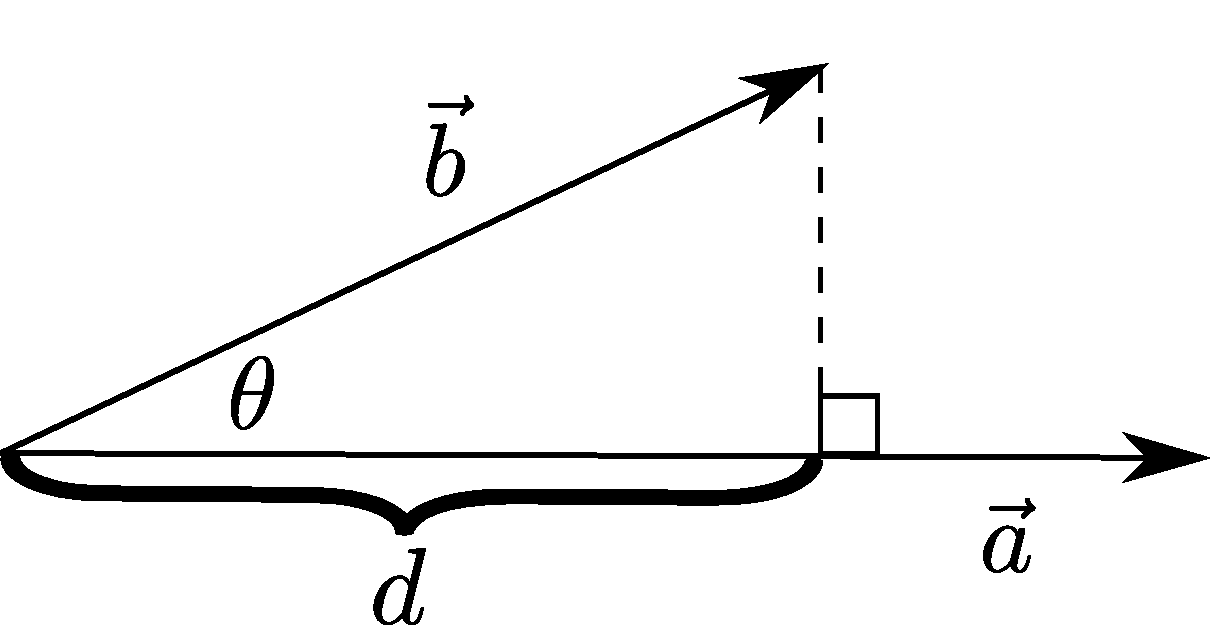
\includegraphics[width=2in]{T3-proj}
    \end{flushleft}
    
    \item Show that
    \[
    (\vec{u}+\vec{v})\dotp (\vec{u}-\vec{v}) = \len{\vec{u}}^2-\len{\vec{v}}^2
    \]
    for any vectors $\vec{u}$, $\vec{v}$ in $\R^3$.
\end{enumerate}
  
\end{document}